\begin{exercises} 

\item Without the aid of a graphing tool match the polynomials to its corresponding graph.
    \begin{flalign*}
        f(x) &= x^3 + 3x^2 - 4x - 12 \\
        g(x) &= -\frac{1}{4}(x-1)^3(x+3) \\
        h(x) &= \frac{1}{3}x^3(x+2)(x-3)^2 \\
        k(x) &= -2x^3-x^2+x
    \end{flalign*}
    \begin{center}
        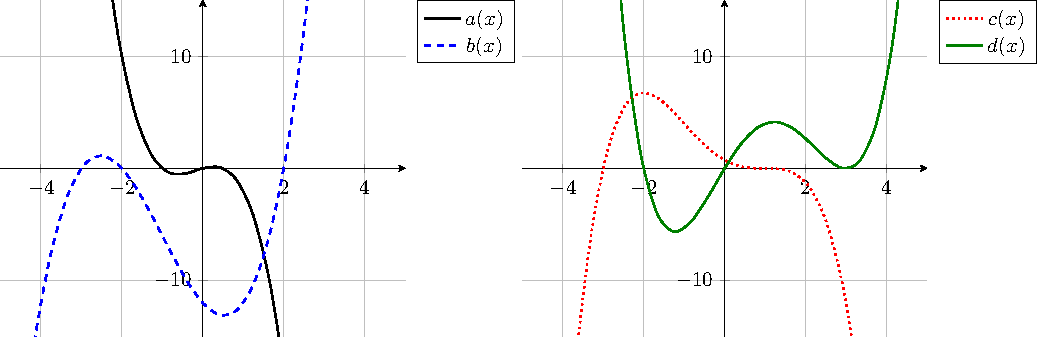
\includegraphics[width=0.99\columnwidth]{figures/0-6-fig6.pdf}
    \end{center}
\begin{exerciseSolution}
\end{exerciseSolution}


\item The cost in dollars for removing $p$ percent of pollutants from a river is 
    \[ C(p) = \frac{61700p}{100-p}. \]
    \ba
        \item Find the cost for removing 20\%.
        \item Find the cost for removing half of the pollutants.
        \item What is the smallest value $p$ can be?
        \item What is the largest value $p$ can be?
        \item What is the value of $C(p)$ as $p \to 100$?  What is the meaning of this in
            the context of the problem?
    \ea
\begin{exerciseSolution}
\end{exerciseSolution}

\item For the function 
    \[ f(x) = \frac{2x-6}{(-6x-1)(6x-6)}, \]
    \ba
        \item what are the vertical asymptotes?
        \item what are the horizontal asymptotes?
        \item what are the coordinates of the $x$ intercepts?
    \ea
\begin{exerciseSolution}
\end{exerciseSolution}

\item Square cuts of the same size are cut from a flat rectangular piece of cardboard. The
    remaining cardboard is folded into a lidless box. Assume that the cardboard originally
    measures 20 inches by 12 inches. Let $x$ be the length of one side of the square cut (at
    this point you should stop and draw a picture).
    \ba
        \item Write a function describing the volume of the resulting box in terms of $x$.
        \item What is an appropriate domain for the volume function?  Plot the volume function
            over the domain.
        \item Write a function describing the surface area of the box in terms of $x$.
        \item Is the domain different for the surface area function?  Why / why not?  Plot
            the surface area function over its appropriate domain.
    \ea

\end{exercises}
\afterexercises
